% !TEX TS-program = pdflatex
% !TEX root = ../XJ_thesis.tex
%

\chapter{Introduction}
\label{sec:intro}

Nowadays, CCD or CMOS cameras are becoming more and more important in many aspects of human life such as photography, security system, and robots, etc. For each camera product, the camera imaging pipeline in the camera is of particular importance since it is the core part to transform the photons reflected by the real scene being captured in the camera sensor into the pixel values of an image, which can be displayed on a screen. During the camera imaging process, the noise is unavoidablely generated due to many reasons. Two major reasons of noise generation are the discrete nature of light and the thermal agitation, which can cause the photon shot noise and the dark-current noise, respectively. Image denoising is the problem of recovering the laten clean image from the captured noise version. 

\textbf{Chapter abstract} This chapter will introduce the image noise and its acquirezation equation, the image denoising problem, the objective measures to evaluate the image denoising performance, the proposed denoising methods. Finally, I will summarize the structural of this thesis, and the contribution I made in this thesis.

%\section{The Camera Imaging Pipeline}
%\label{sec:intro:general}

%The cameras capture the images and store as raw image formats. During the camera imaging pipeline, the photons are transformed into electronics by the photodiode in the camera sensor. The original sensor arrat (also called color filter array, or CFA) contains red, green, and blue channels, and these incomplete channels are transformed into the final RGB files via the raw converter. The camera imaging pipeline includes multiple stages such as reading raw image, black light subtraction, lens correction, demosaicing, noise reduction, white balancing, gamma curve, final color space conversion, etc \cite{browneccv2016}. Basically, a camera imaging pipeline includes demosaicing, white balancing and color space transform, gamut mapping, tone mapping, and JPEG compression \cite{crosschannel2016}. However, different cameras have varying structures and camera parameters, and hence resulting different imaging effects. Recently, there also exists learning based imaging pipelines which directly learn the  natural image priors from the RGB and raw images pairs.


\section{The Formulation of Image Denoising}
\label{sec:intro:current}

Due to the discrete nature of light and the thermal agitation, the camera sensors will cause inaccurate measurement in camera sensors. The inaccurate measurement is also called image noise. The types of image noise generated during the imaging pipeline are mainly the random noise, the spatial non-uniformity noise, and quantization noise. The random noise includes photon shot noise, dark current, and readout noise. The spatial non-uniformity noise includes the fixed pattern noise (PRNU, DCNU), CCD/CMOS specific noise. During the camera imaging pipeline, the noise will be furtherly made complex than those in the raw images.

To better analysis the property of the realistic noise quantitatively, we provide a simplified signal acquisition model \cite{Foipractical} including various noise sources (for each pixel) as follows:
\begin{equation}
\label{e11}
\bm{P} = f((g_{cv}(\bm{C}+\bm{D})+\bm{N}_{reset})g_{out}+\bm{N}_{out})+\bm{Q},
\end{equation}
where $\bm{P}$ is the raw pixel value, $f$ is the camera response function, usually a linear function before attaining a saturation threshold, $\bm{C}$ is the number of absorbed electrons (charges) transformed from the photons via the photon-diodes in the camera sensor, which can be modeled by a Poisson distribution, $\bm{D}$ is the number of absorbed electrons generated by dark current by thermal generation, which is often modeled by a Poisson distribution, $\bm{N}_{reset}$ is the thermal noise generated by the readout circuitry (or reset noise related to reset voltage), which can be well modeled by a Gaussian disribution, $\bm{N}_{out}$ is the readout noise, which is also modeled by a Gaussian distribution, $\bm{Q}$ is the quantization error happened during rounding to interger values, usually uniformly distributed and normally negligible compared to the readout noise, $g_{cv}$ is the equivalent capacitance (EC) of the photo-diode and the gain factor during charge to voltage conversion, $g_{out}$ is the gain factor during voltage to pixel value conversion (readout).

After some merging and simplifying, the signal acquisition model \ref{e11} can be formulated as follows:
\begin{equation}
\label{e12}
\begin{split}
\textbf{P} 
&=f((g_{cv}(\textbf{C}+\textbf{D})+\textbf{N}_{reset})g_{out}+\textbf{N}_{out})+\textbf{Q},
\\
&=f(g_{cv}g_{out}(\textbf{C}+\textbf{D})+g_{out}\textbf{N}_{reset}+\textbf{N}_{out})+\textbf{Q},
\\
&=f(g\lambda+N_{R})+\textbf{Q},
\end{split}
\end{equation}
where $g = g_{cv}g_{out}$ is the overall camera gain factor, $\lambda=\textbf{C}+\textbf{D}$ is number of electrons in pixel capacitor, and $N_{R}=g_{out}\textbf{N}_{reset}+\textbf{N}_{out}$ is the overall readout noise. In summary, the overall noise before the camera imaging pipeline can be modeled by a mixed Poisson and Gaussian distribution \cite{Foipractical}, which can also been approximated by a single Gaussian distribution according to the Central Limit Theorem.

To evaluate the performance of existing image denoising methods, the common type of tested noise is the additive white Gaussian noise (AWGN) \cite{bm3d,ksvd}. The images with AWGN noise are corrupted by random values following Gaussian distribution with zero mean and a certain standard deviation (std). However, the real-world noise in the photographs captured by cameras is very complex and can hardly be modeled by a simple Gaussian distribution. The previous mentioned mixed Poisson and Gaussian distribution \cite{Foipractical} is also an ideal model for the noise in the raw images captured by the cameras. However, due the complex in-camera imaging pipeline, the real-world noise will further become much more complex than those in the raw iamges \cite{crosschannel2016,karaimer_brown_ECCV_2016}. This makes the image denoising, especially the realistic case, still a vary challenging task. The image denoising methods designed for the synthetic AWGN noise may fail when dealing with the realistic images captured by CCD or CMOS cameras.


Image denoising is a classical yet fundamental problem for image quality enhancement in computer vision and photography. In general, image denoising aims to recover the latent clean image $\bm{x}$ from the observed noisy image $\bm{y}=\bm{x}+\bm{n}$, where $\bm{n}$ is assumed to be the additive noise. In literature, most of the existing algorithms are designed for dealing with the additive white Gaussian noise (AWGN), where $\bm{n}$ follows Gaussian distribution $\mathcal{N}(0,\sigma^{2})$.  The AWGN noise is a perfect testing bed for evaluating the image resotration methods for image super-resolution, deblurring, inpainting, etc. However, for realistic cases, the image noise $\bm{n}$ is no longer signal independent, which makes the image denoising problem much more difficult than the AWGN counterpart.


From the perspective of machine learning, image denoising can be viewed as a regression problem, in which a \textsl{plausible} clean image can be obtained from the infinite number of possible candidates. The word \textsl{plausible} means that the denoised image should look like the noisy image but without the noise component. As we know from \cite{Bishop}, regression models, such as the famous least squares regression and LASSO \cite{lasso}, can be very inaccurate if we do not add proper prior to them. Similarly, image denoising problem would be very difficult if we do not employ some suitable prior information on it. One major reason of this difficulty is that we do not know what exactly the latent clean image is without the prior information of the clean image. Hence, it is meaningful to exploit the prior information of the most \textsl{plausible} image given the input noisy image. The most commonly used prior information in image denoising community is the Bayesian rule, which is also known as maximum A-posterior (MAP) property. Under the MAP framework, the most \textsl{plausible} latent clean image is the one with maximum Bayesian probability for its noisy counterpart. The posterior probability can be computed by some explicit form which I will introduce in the following sections. In fact, the posterior probability can measure the distance of the latent clean image to the given noisy image. The closeness is usually measured by an $\ell_{2}$ norm of the difference between the two images mentioned above. There are many latent clean images with the same $\ell_{2}$ norm distance with the given noisy image. But some images in the same distance are more \textsl{plausible} than the others due to the aspects of less artifacts, better structural preservation, and less remaining noise, etc. Hence, besides the MAP property, we need employ further prior information of natural images for better image denoising performance.


In order to evaluate the quality of the denoised images, as well as compare the denoising performance of different methods, we need calculate the measurements of goodness for the denoised images. A natural problem is, how to measure the quality of the denoised image? To answer this question, we need resort to the image quality assessment (IQA) algorithms, which aim to find good solution to measure the image quality for different applications such as image denoising, deblurring, super-resolution, etc. 

For different denoising tasks, we need different image quality assessment algorithms. For the synthetic experiments on additive white Gaussian nosie (AWGN), we have the original clean images for the corresponding denoised images. This is because the noisy image is itself generated by adding synthetic AWGN noise to the corresponding original clean image. Then we can directly measure the quality of the denoised image by some existing IQA metrics. However, the original clean image does not always exists. For the realistic image denoising task, the corresponding clean image is hard to generate. A possible solution is to evaluate the image quality by human subjective. An alternative solution is to generate a latent clean image for objective image quality assessment. According to whether the reference clean image can be provided or not, the existing IQA metrics can be roughly divided into two directions: 1) full reference IQA; and 2) no reference IQA. Full reference IQA metrics are based on the assumption that the true underlying image is available in order to compute a measure, while no reference IQA metrics perform quality assessments without the reference image since the true underlying image is not available. The full reference IQA metrics include root-mean-square error (RMSE), peak signal-to-noise ratio (PSNR), and the structural similarity index (SSIM), etc. Other IQA metrics include the multi-scale SSIM (MS-SSIM), BLIINDS, and BIQI, etc. An detailed survey of existing IQA algorithms is not the major contribution of this thesis. For more references, please refer to \cite{ssim}. Now we introduce briefly the above mentioned IQA metrics as follows:

\textbf{RMSE}: The root mean square error (RMSE) of the denoised image $\bm{y}\in\mathcal{R}^{M\times N}$ w.r.t. the original clean image $\bm{x}\in\mathcal{R}^{M\times N}$ is defined as the square root of the mean square error (MSE). The RMSE is usually employed to measure the distance between the denoised image and the original clean image. It is a full reference IQA metric which is closely related to the following PSNR metric. The definition of RMSE is:
\begin{equation}
\label{e13}
\text{RMSE}(\bm{x},\bm{y})
=
\sqrt{\frac{1}{MN}\sum_{i=1}^{M}\sum_{j=1}^{N}(\bm{x}_{ij}-\bm{y}_{ij})^{2}}.
\end{equation}



\textbf{PSNR}: PSNR is the most commonly used full reference IQA metric for many image restoration tasks including denoising. The definition of PSNR can be formulated as follows (for 8-bit image):
\begin{equation}
\label{e14}
\text{PSNR}
=
20\text{log}_{10}
(\frac{2^{8}}{\text{RMSE}(\bm{x},\bm{y})}).
\end{equation}
As we can see, PSNR is closely related to the $\ell_{2}$ norm distance between two images. The unit of PSNR is decibel (dB) and higher dB value indicates better image quality and lower RMSE. Even thouth PSNR is very simple and intuitive, higher PSNR does not indicate higher visual structural similarity. Hence, many researchers still make effort to find alternative and better IQA metrics. Usually, smaller RSME value indicates better image quality. 

\textbf{SSIM} \cite{ssim}: One seminar work in IQA is the famous structural similarity (SSIM) index metric, which is also a full reference IQA metric. In SSIM, each image patch is decomposited into three different components indicating three core informative parts of the original patch. The three components are luminance (mean value of the pixels in the patch), contrast (the standard deviation of the patch), and structure (the mean subtracted patch). SSIM takes into account the fact that the human visual system is very sensitive to the relative changes in luminance, rather than the absolute changes in luminance. The value range of the SSIM is between 0 and 1, where higher value indicate higher similarity (SSIM=1 indicates that the two images are exactly the same). Usually, higher SSIM value indicates better image quality. 

\textbf{Other IQA Metrics}: Besides of the frequently used RMSE, PSNR and SSIM, there are many other IQA metrics for full reference and no reference IQA. Some examples include the MS-SSIM \cite{msssim}, which is a multi-scale extension of the original SSIM. Some examples in no reference IQA include BLIINDS \cite{bliinds} and BIQI \cite{biqi}. These IQA metrics capture the deviations from the expected statistics of the natural images. For example, BLIINDS measures the deviations from the expected histogram of certain features in DCT domain, while BIQI measures deviations from the expected distribution of wavelet coefficients in a multi-scale decomposition.

I have to mention that no IQA metric is perfect or best for image denoising task, both in full reference and no reference cases. The de facto standard metrics in image restoration community are PSNR and SSIM. In order to avoid these two metrics generate bad results, it is essential to demonstrate the image quality in the thesis for human subjective evaluation.


\section{Existing Denoising Methods}

In this section, I will review the existing methods related to the image denoising literature during the past decades. I will firstly review some widely known image denoising methods designed for additive white Gaussian noise (AWGN), which is the most frequently studied area in the literature. Though the reviewed methods are mainly proposed for the AWGN noise, the idea can be transfered into other image denoising tasks such as realistic image denoising. Then I will review some existing methods proposed for real world noisy images. We believe that the realistic image denoising problem is the current mainstream in the image denoising research. Due to the fact that the noise in real world image cannot be explicitly modeled, noise model assumption and estimation should be given or the real noisy image denoising task. Since the noise is mainly assumed to be Gaussian distributed, I will finally review some state-of-the-art image noise estimation methods in the literature.

\subsection{Synthetic Image Denoising}
\label{sec:review:sys}

Image denoising is a classical problem in low level vision. It has been extensively studied in the past decades, and is still an active research topic for the reason that it provides an ideal test bed for image modeling techniques and other image restoration ideas. In synthetic image denoising problem, image denoising aims to recover the clean image $\mathbf{x}$ from its noisy observation $\mathbf{y} = \mathbf{x} + \mathbf{n}$. $\mathbf{n}$ is the synthetic image noise, which is often assumed to be additive white Gaussian noise (AWGN). Other types of synthetic image noise, e.g., Poisson noise and salt-and-pepper noise, are also been widely studied in literature. The Poisson noise can be transformed into the additive noise after the generalized Anscombe transformation \cite{makitalo2013optimal}. Besides, the salt-and-pepper noise is naturally additive noise and can be naturally formulated into the same model mentioned above.

Amount of image denoising methods have been developed in past decades. The Partial Differential Equation (PDE) based methods such as nonlinear anisotropic diffusion \cite{PeronaMalik1990} define a class of efficient approaches, in which each diffusion step includes only the convolution operation with a few linear filters. The total variation based methods \cite{rudin1992nonlinear,osher2005iterative} have a principle that signals with excessive and possibly spurious detail have high total variation, and hence reducing the total variation of the signal subject to it being a close match to the original signal. This work is pioneered by Rudin, Osher, and Fatemi in 1992, and hence be known as ROF model \cite{rudin1992nonlinear}. It is widely accepted that natural image gradients exhibit heavy-tailed distributions \cite{weiss}, and the total variation (TV) based methods \cite{rudin1992nonlinear,osher2005iterative} actually assume Laplacian distributions of image gradients for denoising. The filtering based methods such as the famous bilateral filter \cite{Tomasi1998} is a non-linear, edge preserving, and smoothing filter for image denoising. It replaces the intensity of each pixel with a weighted average of intensity values from nearby pixels. By modeling the wavelet transform coefficients as Laplacian distributions, many wavelet shrinkage based denoising methods such as the classical soft-thresholding \cite{softthresholding} have been proposed.\ Chang et al. modeled the wavelet transform coefficients as generalized Gaussian distribution, and proposed the BayesShrink \cite{bayesshrink} algorithm. Other curvelet based extensions are also proposed in \cite{curvelet}. By considering the correlation of wavelet coefficients across scales, Portilla et al. \cite{blsgsm} proposed to use Gaussian Scale Mixtures for image modeling and achieved promising denoising performance.  The Fields of Experts (FoE) \cite{foe} proposed by Roth and Black models the filtering responses with Student's t-distribution to learn filters through Markov Random Field (MRF) \cite{Bishop}. The nonlocal means (NLM) \cite{nlm} has a basic idea that to build a pointwise estimate of the image where each pixel is a weighted average of pixels centered at regions that are similar to the region centered at the estimated pixel. Later, the seminar work of K-SVD \cite{ksvd} was introduced in which an overcomplete dictionary is learned for the extracted image patches under the sparse representation framwork \cite{olshausen1997sparse,olshausen1996emergence}. One representative is the sparse representation based scheme which encodes an image patch as a linear combination of a few atoms selected from a dictionary \cite{olshausen1996emergence,olshausen1997sparse,ksvd}. The dictionary can be chosen from the off-the-shelf dictionaries (e.g., wavelets and curvelets), or it can be learned from natural image patches.\ The seminal work of K-SVD \cite{ksvdtsp,ksvd} has demonstrated promising denoising performance by dictionary learning, which has yet been extended and successfully used in various image processing and computer vision applications \cite{srcolor,srcvpr,lcksvd}. By viewing image patches as samples of a multivariate variable vector and considering that natural images are non-Gaussian, Zoran and Weiss \cite{epll,gmmnips} and Yu et al.  \cite{ple} used Gaussian Mixture Model (GMM) to model image patches, and achieved state-of-the-art denoising and image restoration results, respectively. Inspired by the sparse representation based methods such as K-SVD \cite{ksvd}, the seminar work of BM3D is introduced in \cite{bm3d}. The BM3D method groups similar image patches into 3D data arrays, transform the  patches into the wavalet domain, and then collaboratively filter the coefficients via shrinkage, and finally inverse transformation to recover the image. Due to the impressive performance BM3D achieves, the sparse representaion has been widely employed in many different methods \cite{lssc,ncsr} for image denoising and other image restoration problems. Besides, since the nonlocal self-similarity (NSS) property has been demonstrated its effectiveness on image denoising task, low rank based methods \cite{nnm,wnnm} have been proposed to exploit the intrinsic NSS property of nonlocal similar patches. For example, the seminar work of WNNM \cite{wnnm} method achieves state-of-the-art performance for AWGN denoising. Over the last few years, some discriminative denoising methods have also been developed by learning discriminative priors from pairs of clean and noisy images \cite{mlp,csf,tnrd, dncnn}. The multiple layer perception (MLP) \cite{mlp} has been introduced in the image denoising community and achieves effective performance. Later, Schmidt and Roth proposed the cascade of shrinkage fields (CSF) to perform denoising efficiently \cite{csf}. Chen et al. proposed the trainable nonlinear reaction diffusion (TNRD) \cite{tnrd}, which achieves even better performance on image denoising as well as much faster speed. Recently, the residual network \cite{residualnetwork} has been applied into the image denoising task, and the proposed DnCNN method \cite{dncnn} has achieved quite state-of-the-art performance on image denoising.


\subsection{Realistic Color Image Denoising}
\label{sec:review:feature}

The challenges are very different in the color image denoising when compared to the grayscale image denoising problem. When the input noisy image is a noisy RGB color image, there are mainly three strategies for color image denoising. (1) The first strategy is to apply the grayscale image denoising algorithm to each channel. However, such a straightforward solution will not exploit the spectral correlation among RGB channels, and the denoising performance may not be very satisfying. (2) The second strategy is to transform the RGB image into a less correlated color space, such as YCbCr, and perform denoising in each channel of the transformed space \cite{foe,cbm3d}. One representative work along this line is the CBM3D algorithm \cite{cbm3d}. However, the color transform will complicate the noise distribution, and the correlation among color channels is not fully exploited. (3) The third strategy is to perform joint denoising on the RGB channels simultaneously for better use of the spectral correlation. For example, the patches from RGB channels are concatenated as a long vector for processing \cite{mairal2008sparse,Zhu_2016_CVPR}.

Though joint denoising of RGB channels is a more promising way for color image denoising, it is not a trivial extension from single channel (grayscale) image to multiple channels (color) image.\ The noise in standard RGB (sRGB) space can be approximately modeled as AWGN, but it has different variances for different channels \cite{Liu2008,Leungtip,crosschannel2016} due to the sensor characteristics and on-board processing steps in digital camera pipelines \cite{crosschannel2016,karaimer_brown_ECCV_2016}.\ This makes the real color image denoising problem much more complex.\ If the three channels are treated equally in the joint denoising process, false colors or artifacts can be generated \cite{mairal2008sparse}.\ How to account for the different noise characteristics in color channels, and how to effectively exploit the within and cross channel correlation are the key issues for designing a good color image denoising method.

During the last decade, a few methods have been proposed for real color image denoising.\ To the best of our knowledge, the study of real color image denoising can be traced back to the BLS-GSM model \cite{blsgsm}. In \cite{blsgsm}, Portilla et al. proposed to use scale mixture of Gaussian in overcomplete oriented pyramids to estimate the latent clean images. In \cite{fullyblind}, Portilla proposed to use a correlated Gaussian model for noise estimation of each wavelet subband. Based on the robust statistics theory \cite{huber2011robust}, Rabie modeled the noisy pixels as outliers, which could be removed via Lorentzian robust estimator \cite{rabie2005robust}. The CBM3D method \cite{cbm3d} is a representative color image denoising method, which first transforms the RGB image into a luminance-chrominance space (e.g., YCbCr) and then applies the benchmark BM3D method \cite{bm3d} to each channel separately.\ The non-local similar patches are grouped by the luminance channel.\ In \cite{Liu2008}, Liu et al.\ proposed the ``Noise Level Function'' to estimate the noise for each channel in natural images, and then use Gaussian conditional random field to obtain the latent clean image \cite{Liu2008}.\ However, processing each channel separately would often achieve inferior performance to processing the color channels jointly \cite{mairal2008sparse}.\ Later, Lebrun el al. proposed a multiscale denoising algorithm called 'Noise Clinic' \cite{noiseclinic} for blind image denoising task. This method generalizes the NL-Bayes \cite{nlbayes} to deal with signal and frequency dependent noise.\ Therefore, the methods \cite{noiseclinic,ncwebsite,Zhu_2016_CVPR} perform real color image denoising by concatenating the patches of RGB channels into a long vector.\ However, the concatenation treats each channel equally and ignores the different noise statistics among these channels.\ The method in \cite{crosschannel2016} models the cross-channel noise in real noisy images as multivariate Gaussian and the noise is removed by the Bayesian non-local means filter \cite{kervrann2007bayesian}.\ The commercial software Neat Image \cite{neatimage} estimates the noise parameters from a flat region of the given noisy image and filters the noise accordingly.\ The methods in \cite{crosschannel2016,neatimage} ignore the non-local self-similarity of natural images \cite{bm3d,wnnm}. 


Despite the success of these methods, they have many limitations. On one hand, as suggested in \cite{Liu2008,noiseclinic}, Gaussian noise, assumed by \cite{fullyblind,rabie2005robust,Liu2008}, may be inflexible for more complex noise in real images. Hence, better approximation to the noise could bring better image denoising performance \cite{Liu2008,noiseclinic}. Based on these observations, it is still needed to design an robust and effective model for blind image denoising. Few assumption and no parameter tuning would bring extra points.


\section{Contribution and Thesis Organization}
\label{sec:intro:new}
\begin{figure}
\centering
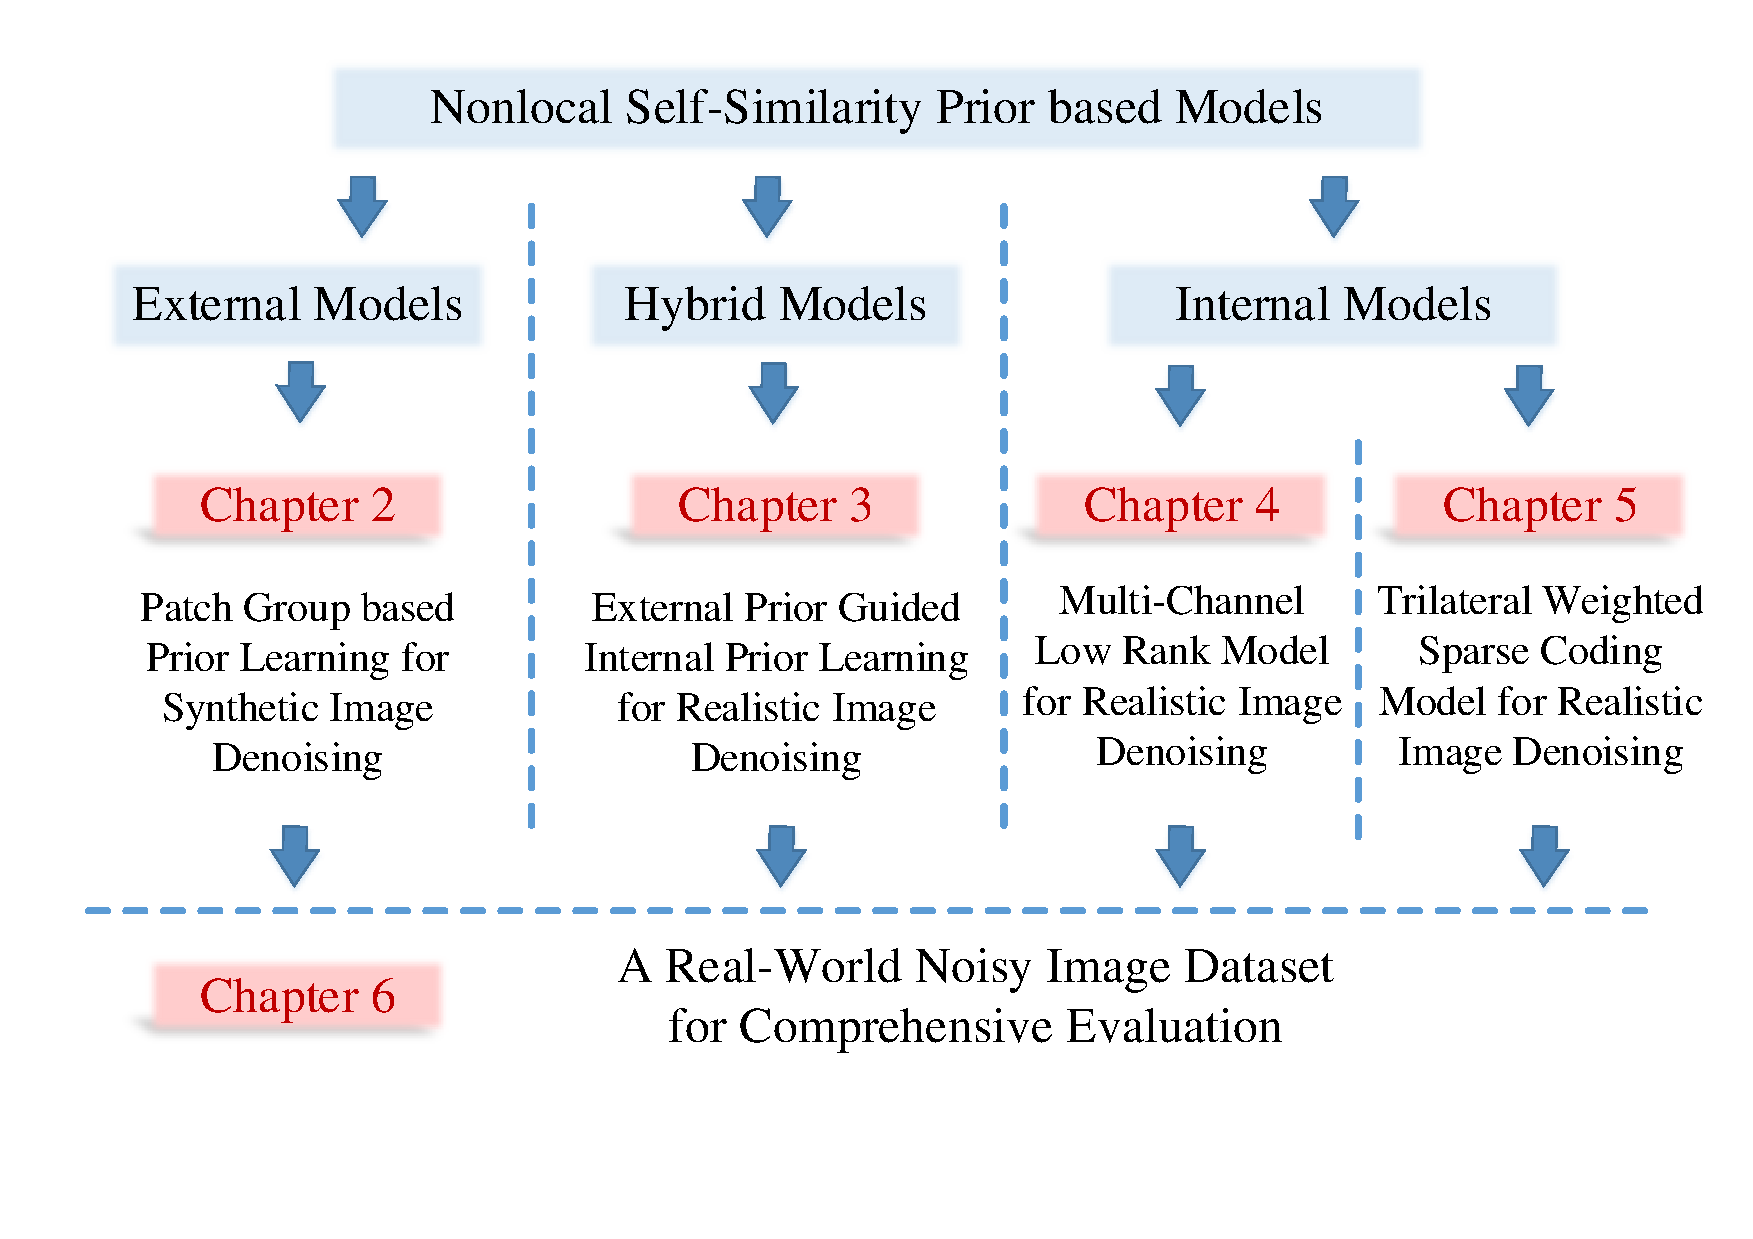
\includegraphics[width=1\linewidth]{images/ThesisOrganization.pdf}
\caption{The organization of this thesis.}
\label{fig1-1}
\end{figure}

This thesis is mainly consisted of five projects I have done during my PhD study, during which I focus on designing new and better image denoising algorithms, aiming at proposing cutting-edge techniques for image denoising and image modeling. The organization of the thesis is illustrated in Figure 1.1.

\textbf{In the first work}, I propose to learn the external NSS priors and apply the learned model on denoising AWGN noise. This is very different to the previous methods, which can be divided into three types: exploiting internal patch prior based methods \cite{ksvd,ple}, exploiting internal NSS prior based methods \cite{bm3d,lssc,ncsr,wnnm}, and learning external patch prior based methods \cite{epll}. The proposed method achieves state-of-the-art performance on AWGN denoising on both effectiveness and efficiency. Basing on the success on the synthetic noise removal, I propose to exploit the power of the NSS priors in natural images to deal with the complex realistic noise in real-world noisy images. Specifically, we propose three methods exploiting the NSS priors of natural images for real noisy image denoising, which can be introduced as follows.

\textbf{In the second work}, I propose to learn the NSS prior from the external natural images, and then apply the learned external prior to guide the learning of the internal NSS prior of the input real noisy image. The experiments on two commonly used datasets and a new one we constructed to implement the shortage of existing datasets, demonstrate that the proposed method can achieve better performance than existing color image denoising methods such as CBM3D \cite{cbm3d}, the state-of-the-art Gaussian noise removal methods \cite{bm3d,mlp,csr}, and the real noisy image denoising methdos \cite{} including a commercial software Neat Image \cite{neatimage}, which is embeded into the famous PhotoShop CS for image processing tasks.


\textbf{In the third work}, I propose to employ the low rank model describe fully the the internal NSS prior, basing on the observed fact that the similar image patches can be contanated as a matrix of low rank. Different from the previous work, I extend the WNNM model and apply it to multi-channel version to make it feasible for color image denoising. 


\textbf{In the fourth work}, I propose to use the sparse coding based method with additional weighting scheme to regard the local noise in real noisy images as a Gaussian and the prior is used to deal with the real noisy image.


\textbf{In the final work}, to make my thesis more comprehensive, I construct a large benchmark of real noisy images captured by different types of famous commercial cameras, on which I also evaluate the image denoising methods mentioned above and the proposed methods in this thesis. 


The structure of this thesis is organized as follows: in the chapter 2, we introduce the fully external method; in the chapter 3, we introduce the external prior guided internal method; in the chapter 4, we introduce the internal method based on low ran model; in the chapter 5, we introduce the internal method based on sparse coding model; in the chapter 6, we introduce the real noisy image dataset we construct, and finaly evaluate the proposed methods with the compared competing methods, both for synthetic AWGN or Poisson noise and real noise, including the commercial software designed especially for real noise. 


\section{Thesis Structure}
\label{sec:intro:structure}


%\textbf{Chapter \ref{sec:review}: Literature Review} \\[0.2em]

%In this chapter, we review the related work and give a detailed introduction of the literature. We will first review the most representative work on additive white Gaussian noise removal. I review the detailed work on camera imaging pipeline and realistic noise generated in the camera sensors. I will also review the work on real noisy image denoising.



\textbf{Chapter \ref{sec:external}: External Nonlocal Self-Similarity Prior Learning for Synthetic Gaussian Noise Removal} \\[0.2em]

In this chapter, I will introduce our work on external nonlocal self-similarity (NSS) prior learning for synthetic Gaussian noise removal. As far as we know, this work is the first to learn the NSS priors of natural clean images, while previous work only utilize the NSS priors of input noisy image for online denoising. The advantages of this offline learning is that it can preserve the details of natural images while being much faster then most online denoising methods.


\textbf{Chapter \ref{sec:guided}: External Prior Guided Internal Prior Learning for Real Noisy Image Denoising} \\[0.2em]

In this chapter, I will introduce our work on external prior guided internal prior learning method for real noisy image denoising. This work can maintain the advantages of both sides: from the external perspective, the method can preserve the structures of natural images better than the internal methods, while from the perspective of internal method, the proposed method can recover the details of the input noisy image better than the external methods.



\textbf{Chapter \ref{sec:internallr}: Multi-channel Weighted Nuclear Norm Minimization for Real Color Image Denoising} \\[0.2em]

In this chapter, we introduce a multi-channel weighted nuclear norm minimization (MC-WNNM) method. This method regards different channels in RGB images differently to adaptively process the real color noisy images. Besides, this work also propose a new strategy for color image denoising. Experiments demonstrate that the proposed method can achieve better performance on real color image denoising than existing state-of-the-art methods, including some commercial software.



\textbf{Chapter \ref{sec:internalsc}: A Triple Weighted Sparse Coding Scheme for Realistic Noisy Image Denoising} \\[0.2em]

In this chapter, I introduce a novel sparse coding based method for real color image denoising. In this method, I regard the noise in each of the local region in the real noisy image as a Gaussian, and propose a triplely weighted scheme to deal with the complex realistic noise in real color noisy images. Experiments show that the proposed method performs better and faster than the nuclear norm based method mentioned in previous chapter.


\textbf{Chapter \ref{sec:dataset}: A Benchmark on Real Color Noisy Image, with Comprehensive Evaluation of State-of-the-art} \\[0.2em]

To fully boost the research of real color noisy image denoising, we construct a large benchmark on real color noisy images. This dataset is collected from several representative cameras with comprehensive settings on contents, lighting, ISO, shutter, and aperture, etc. Based on this newly established dataset, we fully evaluated existing denoising methods, including the methods designed for synthetic Gaussian noise and the methods designed especially for real color noise. We believe that this new dataset will largely boost the research of the image denoising especially the realistic image denoising problems.





